\graphicspath{{chapters/01/}}
\chapter{Introduction: from classical to quantum}
\section{Classical computing}
Classical computers are made by 
\begin{itemize}
	\item Elementary units: \textbf{bits}, that can take values $0,1$;
	\item Elementary operations carried out by \textbf{logical gates}.
\end{itemize}
Examples of the usage of these two elements are the
\begin{itemize}
 \item The NOT gate 
	 \begin{figure}[H]
 		\centering
		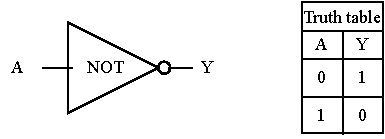
\includegraphics[width=0.35\textwidth]{not.pdf}
	\end{figure}
 \item The AND gate
 	\begin{figure}[H]
 		\centering
		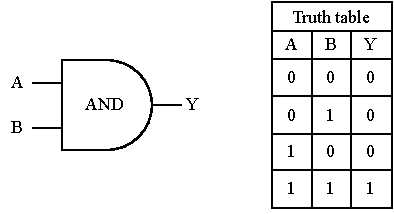
\includegraphics[width=0.35\textwidth]{and.pdf}
	\end{figure}
 \item The NAND gate
 	\begin{figure}[H]
 		\centering
		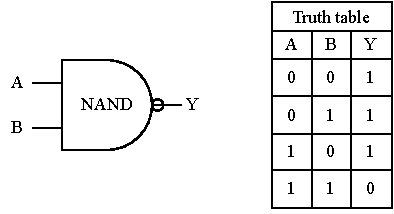
\includegraphics[width=0.35\textwidth]{nand.pdf}
	\end{figure}
\end{itemize}

\subsubsection{Universality and Turing machine}
The concept of universality yields a set of elementary objects that can do all sort of comptutation inside a classical computer. The NAND gate with the copy procedue are togheter universal gates, since all gates can be cosntructed from these two. \\
In the pictures below the construction of the NOT and AND gate are depicted, using ongli the copy and the NAND. 
\begin{figure}[h]
 		\centering
		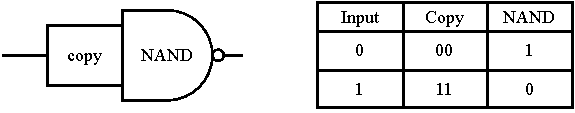
\includegraphics[width=0.5\textwidth]{universal_not.pdf}
	\end{figure}
\begin{figure}[h]
 		\centering
		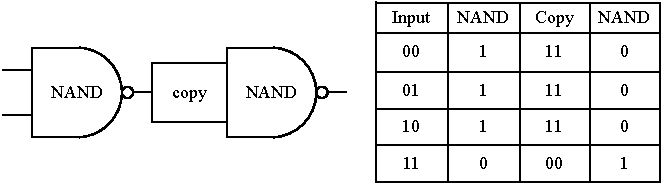
\includegraphics[width=0.5\textwidth]{universal_and.pdf}
	\end{figure}
	
Since the NAND and copy operations can be used to describe all sort of (classical) computations, they also provide for the costruction of the Turing machine. \\
A Turing machine is a mathematical model of computation that defines an abstract machine that manipulates symbols on a strip of tape according to a table of rules.Despite the model's simplicity, given any computer algorithm, a Turing machine capable of implementing that algorithm's logic can be constructed\footnote{\href{https://en.wikipedia.org/wiki/Turing_machine}{wikipedia/Turing\_Machine}}.\\
\begin{figure}[h]
 		\centering
		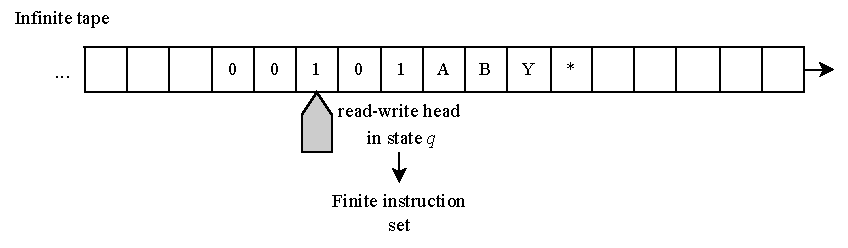
\includegraphics[width=0.5\textwidth]{turing.pdf}
	\end{figure}
	
The machine operates on an infinite memory tape divided into discrete "cells". The machine positions its "head" over a cell and reads the symbol there. The read/write head is now in state \textit{q}. Given the state \textit{q} and the symbol, the machine proceeds with the given finite instruction set: modifies the symbol, the head moves and \textit{q} is adapted. Based on the observed symbol and the machine's own state, either proceeds to another instruction or halts computation.\\
However, the very same definition of the turing machine proves the existance of its fundamental limits. For example, it cannot solve for problems that are not deducidable. The \textit{halting problem} is a well known case: it states that it does not exist an algorithm \textit{f} that cand etermine for any other agorithm \textit{g} if \textit{g} will eventually terminate or run forever. Algorithm \ref{alg:one} shows as an absurd an algorithm \textit{f} that checks wether \textit{g} terminates:

\begin{algorithm}
\caption{f(algorithm g)}\label{alg:one}
\If{$f(g) = terminate$}
{
    \While{true}{
    end}
}\Else{\Return}
\end{algorithm}
Not only that, but also finite resources is another restriction. For example, factorizing prime number is extremely hard (as we'll see later, it is in fact NP) and for this this reason many cryptographic protocols are based on the difficulty of factoring large composite integers or a related problem—for example, the RSA problem. \\
However, Shor's (quantum) algorithm can find the prime factors of an integer in polynomial time. Subsequently, a quantum computer with sufficient number of qbits (and the ability not to succumb any dechorence phenomena) could break RSA and other cryptographic schemes.\\ 

\section{Quantum computing}
As classical computers have bits as fundamental units, quantum ones have \textbf{quantum bits}, or \textbf{qbits} as the basic unit of quantum information. The quantum version of the classical bit is physically realized with a two-state device. 
\subsection{Qbits}
There are two possible outcomes for the measurement of a qubit—usually taken to have the value "0" and "1", like a bit or binary digit. However, whereas the state of a bit can only be either 0 or 1, the general state of a qubit according to quantum mechanics can be a coherent superposition of both. Moreover, whereas a measurement of a classical bit would not disturb its state, a measurement of a qubit would destroy its coherence and irrevocably disturb the superposition state. It is possible to fully encode one bit in one qubit\footnote{\href{https://en.wikipedia.org/wiki/Qubit}{Wikipedia/Qubit}}.\\
\subsubsection{Qbit states}
In quantum mechanics, the general quantum state of a qubit can be represented by a linear superposition of its two orthonormal basis states (or basis vectors). These vectors are usually denoted as
\begin{equation}
\ket{0} = \begin{bmatrix}
           1\\
           0
           \end{bmatrix}
\,\,\,
\ket{1} = \begin{bmatrix}
           0\\
           1
           \end{bmatrix}
\end{equation}
	
	
	
	
	
	
	
	
	
	
	
	
	
	
	
	